\documentclass{article}
%------------------------- packages -------------------------%
\usepackage[vietnamese.licr]{babel}
\usepackage{listings}
\usepackage{tvietlistings}
\usepackage[T1]{fontenc}
\usepackage[utf8]{inputenc} % Đảm bảo sử dụng mã hóa UTF-8
\usepackage{float}
\usepackage[many]{tcolorbox}
\usepackage[unicode,hidelinks]{hyperref}    % for reference
\usepackage{geometry}   % for layout
\usepackage{amsmath}    % for math
\usepackage{xcolor}     % for color
% for figure
\usepackage{graphicx}
\usepackage{caption}    
% for code
\usepackage{minted}
\usepackage[normalem]{ulem}
% for table
\usepackage{xparse}
\usepackage{float}      
\usepackage{paracol}
\usepackage{array}
\usepackage{multirow}
\usepackage{enumitem}
% for header & footer 
\usepackage{fancyhdr}
\usepackage{lastpage}
\usepackage{CJKutf8}
\usepackage{xcolor}


%------------------------- set up -------------------------%
% figure
\graphicspath{{./Images/}}              % path to image
\captionsetup[figure]{labelfont={small,bf,it},textfont={small,it}}
% paragraph
\setlength{\parindent}{0pt}
\setlength{\parskip}{12pt}
\setlength{\parskip}{6pt}               % disables indentation
\renewcommand{\baselinestretch}{1.5}    % line spacing

% code
\def\code#1{\texttt{#1}}    % font
\usemintedstyle{vs}         % minted theme
\setminted{
    autogobble,             % remove all common leading whitespace
    baselinestretch=1.0,
    bgcolor=gray!5!white,
    breaklines,
    %linenos,               % enables line numbers
    fontsize=\footnotesize
}
% Table addrow Macro with dyanamic
% Define the new addrow command to accept a variable number of arguments
\NewDocumentCommand{\addrow}{>{\SplitList{;}}m}{%
  \processline#1\relax
}


% Define a custom style
\lstdefinestyle{myStyle}{
    frame=l,
    framesep=4.5mm,
    framexleftmargin=2.5mm,
    basicstyle=\ttfamily\footnotesize,
    captionpos=b,
    commentstyle=\color{comment},
    breakatwhitespace=false,         
    breaklines=true,                 
    keepspaces=true,                 
    numbers=left,       
    numbersep=5pt,                  
    showspaces=false,                
    showstringspaces=false,
    showtabs=false,                  
    tabsize=2,
    keywords={if, else, for, while, repeat, function, in, next, break, library, ifelse, select, return, print, mutate, hist, tapply, apply, sapply, boxplot, barplot, factor},
		% keywordstyle=\color{blue}\bfseries,
        keywordstyle=\color{comment},
		ndkeywords={class, data.frame, numeric, matrix, character, list, c, seq},
		ndkeywordstyle=\color{black}\bfseries,
		identifierstyle=\color{black},
		sensitive=false,
		comment=[l]{\#},
}
% Helper macro to process each item
\newcommand{\processline}[1]{%
  \ifx\relax#1\relax % End of the list
    \\ \hline
  \else
    #1%
    \expandafter\processnext
  \fi
}

\newcommand{\processnext}[1]{%
  \ifx\relax#1\relax % End of the list
    \\ \hline
  \else
    & #1%
    \expandafter\processnext
  \fi
}

% Callout
\definecolor{main}{HTML}{5989cf}    % setting main color to be used
\definecolor{comment}{HTML}{606060}
\definecolor{sub}{HTML}{cde4ff}     % setting sub color to be used
\newtcolorbox{boxH}{
    % fontupper = \bf,
    boxrule = 1.5pt,
    colback = white, 
    colframe = black % frame color
}
% End
%------------------------- layout & margin -------------------------%
\geometry{
    a4paper,        % redundant if already in \documentclass
    left=20.32mm,
    right=20.32mm,
    top=25.40mm,
    bottom=25.40mm,
    heightrounded,  % better use it
}
\setlength{\parindent}{20pt}
%------------------------- header & footer -------------------------%
\renewcommand{\headrulewidth}{0.5pt}
\renewcommand{\footrulewidth}{0.5pt}
\setlength{\headheight}{24.5pt}
\pagestyle{fancy}

\fancyhead{}    % clear all header fields
\fancyhead[L]{
    \begin{tabular}{ll}
        \begin{picture}(10,10)
            \put(0,-7){
\includegraphics[width=8mm]{{Images/bachkhoa_logo.png}}}
        \end{picture}&
    	\begin{tabular}{l}
    	    {\ttfamily Trường Đại học Bách Khoa Tp. Hồ Chí Minh} \\
    	    {\ttfamily Khoa Khoa học và Kỹ thuật Máy tính} \\
    	\end{tabular} 	
    \end{tabular}
}

\fancyfoot{}    % clear all footer fields
\fancyfoot[L]{\footnotesize {\ttfamily Báo cáo bài tập lớn Xác Suất Thống Kê Kì 243}}
\fancyfoot[R]{\footnotesize {\ttfamily Trang {\thepage}/\pageref{LastPage}}}
% might change to \scriptsize

%------------------------- body -------------------------%
\begin{document}


% Use \lstset to make myStyle the global default
\lstset{style=myStyle}
%-------------------- cover --------------------%
\begin{titlepage}
\begin{center}
    \large ĐẠI HỌC QUỐC GIA THÀNH PHỐ HỒ CHÍ MINH \\
    TRƯỜNG ĐẠI HỌC BÁCH KHOA \\
    KHOA KHOA HỌC VÀ KỸ THUẬT MÁY TÍNH
\end{center}

\vspace{1.5cm}

\begin{figure}[!ht]
    \centering 
\includegraphics[width=3.5cm]{Images/bachkhoa_logo.png}
\end{figure}

\vspace{1.5cm}

\begin{table}[H]
    \centering
    \begin{tabular}{c}
    {\bf \Large XÁC SUẤT THỐNG KÊ (MT2013)} \\ \\
    \hline  \\
    \multicolumn{1}{l}{{\bf \large Báo cáo Bài tập lớn}}    \\  \\
    {\bf \huge THỐNG KÊ DỮ LIỆU BÁN LẺ GIAO DỊCH}     \\  
    {\bf \huge  CỦA CỬA HÀNG ĐIỆN TỬ}     \\  \\
    \hline
    \end{tabular}
\end{table}

\vspace{1.5cm}

\begin{table}[h]
\centering
\begin{tabular}{lrlc}

\hspace{0 cm} & GVHD: Cô Nguyễn Kiều Dung & \vspace{0.5cm}\\
& SV thực hiện: &  
 	
    Bùi Nguyễn Hoàng Thọ& 2333017\\
& & Trần Văn Được& 2210782\\
& & Trịnh Duy Nghiêm & 2312256\\

\end{tabular}
\textbf{\textit{}}\end{table}

\vspace{1.0cm}

\begin{center}
    \footnotesize Tp. Hồ Chí Minh, Tháng 8/2025
\end{center}
\end{titlepage}
\newpage
\textbf{Tên nhóm: MT01}
\begin{table}[H]
\centering
\begin{tabular}{|c|l|l|l|l|}
\hline
\textbf{STT} & \textbf{Họ tên SV} & \textbf{MSSV} & \textbf{Tên lớp} & \textbf{Ngành / Khoa} \\
\hline
1 & \textbf{Bùi Nguyễn Hoàng Thọ} & 2333017 & DT03 & KH-KT máy tính \\
\hline
2 & Trần Văn Được & 2210782 & DT03 & Điện - Điện tử \\
\hline
3 & Trịnh Duy Nghiêm & 2312256 & DT03 & KH-KT máy tính \\
\hline

\end{tabular}
\label{tab:motadonggoptungthanhvien}
\end{table}

\newpage
%-------------------- mission --------------------%
%\renewcommand{\arraystretch}{2}

%-------------------- mục lục --------------------%
\tableofcontents
%-------------------- Chia các mục --------------------%
\section*{\begin{center}
\Huge{Giới thiệu}
	\end{center}}

Trong thời đại khoa học công nghệ phát triển mạnh mẽ, nhu cầu sử dụng linh kiện và thiết bị điện tử ngày càng gia tăng. Điều này đã đặt ra yêu cầu cao hơn về chất lượng sản phẩm và dịch vụ, buộc các cửa hàng điện tử phải đối mặt với sự cạnh tranh khốc liệt. Để thu hút và giữ chân khách hàng, nhiều chương trình khuyến mãi cùng các chính sách ưu đãi được triển khai liên tục, đáp ứng tốt hơn nhu cầu và nâng cao chất lượng đời sống người tiêu dùng.

Để đạt được những mục tiêu này, các cửa hàng điện tử không ngừng đầu tư vào việc phân tích dữ liệu giao dịch bán lẻ. Đây là một bước quan trọng, giúp khảo sát nhu cầu khách hàng, từ đó xây dựng các chiến lược kinh doanh hiệu quả và tối ưu hóa phương thức tiếp cận thị trường.

Với mong muốn có một góc nhìn tổng quát hơn về hoạt động phân tích trong kinh doanh, chúng em đã chọn đề tài “Thống kê dữ liệu bán lẻ giao dịch của cửa hàng điện tử”. Qua đó, chúng em hy vọng có thể tự mình thử nghiệm và áp dụng các kiến thức về xác suất và thống kê đã được tích lũy trong quá trình học tập.

Trong quá trình thực hiện báo cáo, nếu có bất kỳ thiếu sót nào, nhóm rất mong nhận được sự góp ý từ thầy để hoàn thiện tốt hơn.

 \newpage

 
\section{Tóm Tắt Dữ Liệu}

\subsection{Ngữ cảnh}
Bộ dữ liệu được sử dụng lấy từ Kaggle, mô phỏng các giao dịch bán lẻ tại một cửa hàng điện tử. Nó chứa thông tin chi tiết về đơn hàng, khách hàng, sản phẩm mua, và phản hồi của khách hàng.

\subsection{Cách dữ liệu được thu thập}
Bộ dữ liệu trên là tổng hợp những đơn hàng sản phẩm đã được thanh toán tại một cửa hàng điện tử. Nó đi kèm với ngày thanh toán, thông tin sản phẩm, và thông tin khách hàng.

\subsection{Các loại biến và quan trắc}
Nhóm đã tổng hợp lại được tổng cộng 1,000 giá trị quan trắc liên quan đến các giao dịch và 3 giá trị liên quan đến thông tin các kho hàng.

Trong quá trình tổng hợp, các biến trong bộ dữ liệu được đưa ra như sau:
\begin{itemize}
    \item \textbf{Biến định tính (Categorical variables):}
    \begin{itemize}
        \item \texttt{order\_id}: Mã đơn hàng.
        \item \texttt{customer\_id}: ID khách hàng.
        \item \texttt{nearest\_warehouse}: Tên kho hàng gần nhất.
        \item \texttt{season}: Mùa trong năm.
        \item \texttt{latest\_customer\_review}: Nhận xét từ khách hàng.
        
    \end{itemize}
    \item \textbf{Biến định lượng (Numerical variables):}
    \begin{itemize}
        \item \texttt{order\_price}: Giá trị đơn hàng trước khuyến mãi.
        \item \texttt{delivery\_charges}: Phí giao hàng.
        \item \texttt{coupon\_discount}: Giá trị khuyến mãi áp dụng.
        \item \texttt{order\_total}: Giá trị đơn hàng sau khuyến mãi.
        \item \texttt{customer\_lat} và \texttt{customer\_long}: Vĩ độ và kinh độ của khách hàng.
        \item \texttt{distance\_to\_nearest\_warehouse}: Khoảng cách đến kho gần nhất.
    \end{itemize}
    \item \textbf{Biến Boolean:}
    \begin{itemize}
        \item \texttt{is\_expedited\_delivery}: Có giao hàng nhanh hay không.
        \item \texttt{is\_happy\_customer}: Khách hàng hài lòng hay không.
    \end{itemize}
\end{itemize}
\raggedbottom
\section{Cơ sở lý thuyết (Kiến thức nền)}

\subsection{Giới thiệu về công cụ sử dụng thống kê}

\subsubsection{Ngôn ngữ R}
R là một công cụ rất mạnh cho học máy, thống kê và phân tích dữ liệu. Nó là một ngôn ngữ lập trình, có thể sử dụng trên bất kỳ hệ điều hành nào do tính chất độc lập nền tảng (\textit{platform-independent}). R có khả năng tích hợp với các ngôn ngữ khác như C, C++ và cho phép tương tác với nhiều nguồn dữ liệu cũng như các gói thống kê như SAS, SPSS.

\subsubsection{Công cụ RStudio}
RStudio là một môi trường phát triển tích hợp (IDE - Integrated Development Environment) dành riêng cho R. RStudio cung cấp giao diện trực quan và các chức năng thuận tiện để làm việc với R mà không cần chạy R trực tiếp.

\subsection{Các khái niệm về thành phần và phương pháp sử dụng thống kê}

\subsubsection{Biến định lượng}
Biến định lượng là những biến có thể đo lường được bằng các con số và thực hiện các phép toán số học như cộng, trừ, nhân, chia. Biến định lượng cung cấp thông tin về "mức độ" hoặc "số lượng" của một đặc điểm cụ thể.

\subsubsection{Phân phối chuẩn}

\textbf{Khái niệm:}  
Phân phối chuẩn, còn gọi là phân phối Gauss (theo tên nhà toán học Carl Friedrich Gauss), là một loại phân phối liên tục. Đặc điểm nổi bật của phân phối chuẩn là:
\begin{itemize}
    \item Đối xứng qua giá trị trung bình.
    \item Có hình dạng chuông.
    \item Các giá trị được phân bố đều xung quanh trung bình và giảm dần khi xa trung bình.
\end{itemize}

\subsubsection{ Kiến thức thống kê mô tả}

\paragraph{Các chỉ số đo lường xu hướng tập trung:}
\begin{itemize}
    \item \textbf{Trung bình (Mean):} Là giá trị trung tâm của bộ dữ liệu, được tính bằng công thức:
    \[
    \text{Mean} = \frac{\sum x_i}{n}
    \]
    trong đó $x_i$ là các giá trị quan sát, $n$ là số lượng giá trị.
    \item \textbf{Trung vị (Median):} Là giá trị nằm ở giữa khi các giá trị được sắp xếp theo thứ tự tăng dần.
    \item \textbf{Mốt (Mode):} Là giá trị xuất hiện nhiều nhất trong bộ dữ liệu.
\end{itemize}

\paragraph{Các chỉ số đo lường sự phân tán}
\begin{itemize}
    \item \textbf{Phương sai (Variance):} Đo lường mức độ phân tán của dữ liệu xung quanh giá trị trung bình, được tính bằng công thức:
    \[
    \text{Variance} = \frac{\sum (x_i - \bar{x})^2}{n}
    \]
    \item \textbf{Độ lệch chuẩn (Standard Deviation):} Là căn bậc hai của phương sai:
    \[
    \text{SD} = \sqrt{\text{Variance}}
    \]
    \item \textbf{Khoảng (Range):} Là hiệu giữa giá trị lớn nhất và giá trị nhỏ nhất trong bộ dữ liệu.
\end{itemize}

\paragraph{Các chỉ số mô tả sự phân bố}
\begin{itemize}
    \item \textbf{Tứ phân vị (Quartiles):} Là các giá trị chia dữ liệu thành bốn phần bằng nhau.
    \item \textbf{Khoảng tứ phân vị hay độ khoảng giữa (Interquartile Range - IQR):} Là khoảng cách giữa tứ phân vị thứ ba ($Q_3$) và tứ phân vị thứ nhất ($Q_1$), được tính bằng:
    \[
    \text{IQR} = Q_3 - Q_1
    \]
\end{itemize}

IQR là một chỉ số quan trọng giúp xác định sự phân tán dữ liệu và phát hiện các giá trị ngoại lai (outliers). Các giá trị được coi là ngoại lai nếu nằm ngoài khoảng:
\[
[Q_1 - 1.5 \times \text{IQR}, Q_3 + 1.5 \times \text{IQR}]
\]

\paragraph{Biểu đồ sử dụng thống kê}
\begin{itemize}
    \item \textbf{Biểu đồ cột (Barplot):} Dùng so sánh các giá trị khác nhau.
    \item \textbf{Biểu đồ hộp (Box plot):} Thể hiện các tứ phân vị và phát hiện giá trị ngoại lai.
    \item \textbf{Biểu đồ Q-Q (Quantile-Quantile plot):} Kiểm tra dữ liệu có tuân theo phân phối chuẩn hay không.
    \item \textbf{Biểu đồ corrplot}: thể hiện sự tương quan của dữ liệu. 
\end{itemize}

\subsection{Kiến thức thống kê suy luận (Tóm tắt)}
% Lý thuyết kiểm định
\subsubsection{Lý thuyết Kiểm định thống kê}
\begin{boxH}
    \textbf{Kiểm định} là quá trình sử dụng dữ liệu mẫu để đưa ra quyết định về một giả thuyết nào đó liên quan đến tổng thể.
  \begin{itemize}
    \item \textbf{Giả thuyết không (Null Hypothesis - $H_0$):} Giả thuyết ban đầu cho rằng không có sự khác biệt hoặc mối quan hệ nào giữa các biến.
    \item \textbf{Giả thuyết thay thế (Alternative Hypothesis - $H_1$):} Giả thuyết cho rằng có sự khác biệt hoặc mối quan hệ giữa các biến.
    \item \textbf{Mức ý nghĩa (Significance Level - $\alpha$):} Xác định ngưỡng để bác bỏ giả thuyết không, thường là 0.05 hoặc 0.01.
    \item \textbf{Giá trị p (p-value):} Xác suất để quan sát được dữ liệu mẫu nếu giả thuyết không là đúng. Nếu p-value nhỏ hơn mức ý nghĩa $\alpha$, ta bác bỏ giả thuyết không.
  \end{itemize}
\end{boxH}
\subsubsection{Kiểm định z-test cho 1 mẫu}

\subsubsection{Kiểm định t-test cho 2 mẫu độc lập}
\begin{itemize}
    \item \textbf{Định nghĩa:} Kiểm định t-test là một phương pháp thống kê dùng để so sánh trung bình của hai nhóm độc lập hoặc hai mẫu liên quan nhằm xác định xem có sự khác biệt có ý nghĩa thống kê giữa chúng hay không.
    \item \textbf{Ý nghĩa:}
    \begin{itemize}
        \item Phù hợp cho dữ liệu có phân phối tuỳ ý và mẫu lớn ($ n> 30 $)
        \item Giúp xác định xem hai nhóm có khác biệt về trung bình hay không.
    \end{itemize}
\end{itemize}
\begin{boxH}
    \textbf{Công thức tổng quát} cho hai mẫu độc lập:
    \[
T = \frac{\bar{X}_1 - \bar{X}_2}{\sqrt{ \frac{s_1^2}{n_1} + \frac{s_2^2}{n_2} }}
\]

\noindent Trong đó:

\begin{itemize}
    \item \( \bar{X}_1, \bar{X}_2 \): trung bình mẫu của hai nhóm (ví dụ: mùa xuân và mùa hè)
    \item \( s_1, s_2 \): độ lệch chuẩn mẫu của hai nhóm
    \item \( n_1, n_2 \): kích thước mẫu của hai nhóm
\end{itemize}

Bậc tự do (degrees of freedom) được ước lượng theo công thức Welch–Satterthwaite:

\[
df = \frac{\left( \frac{s_1^2}{n_1} + \frac{s_2^2}{n_2} \right)^2}{\frac{ \left( \frac{s_1^2}{n_1} \right)^2 }{n_1 - 1} + \frac{ \left( \frac{s_2^2}{n_2} \right)^2 }{n_2 - 1}}
\]

So sánh giá trị \( |T| \) với ngưỡng \( t_{\alpha/2, df} \) để đưa ra kết luận.
\end{boxH}
\subsubsection{Kiểm định Kruskal-Wallis}  
\begin{itemize}
    \item \textbf{Định nghĩa:} Kiểm định phi tham số dùng để so sánh trung vị của \textbf{ba hoặc nhiều nhóm độc lập} nhằm xác định xem có sự khác biệt đáng kể giữa các nhóm khi dữ liệu không theo phân phối chuẩn.  
    \item \textbf{Ý nghĩa:}  
    \begin{itemize}
        \item Phù hợp cho dữ liệu không chuẩn hoặc dữ liệu thứ bậc.  
        \item Kiểm tra sự khác biệt trung vị giữa các nhóm độc lập.  
    \end{itemize}
\end{itemize}

\subsubsection{Kiểm định Wilcoxon-Mann-Whitney}  
\begin{itemize}
    \item \textbf{Định nghĩa:} Kiểm định phi tham số dùng để so sánh \textbf{hai mẫu độc lập}, kiểm tra xem hai mẫu có cùng phân phối hay không.  
    \item \textbf{Ý nghĩa:}  
    \begin{itemize}
        \item Thích hợp khi dữ liệu không chuẩn hoặc có ngoại lệ lớn.  
        \item Ứng dụng cho dữ liệu định lượng hoặc thứ bậc để kiểm tra sự khác biệt về phân phối.  
    \end{itemize}
\end{itemize}

\subsubsection{Kiểm định Wilcoxon Signed-Rank}  
\begin{itemize}
    \item \textbf{Định nghĩa:} Kiểm định phi tham số dùng để so sánh trung vị của \textbf{hai tập dữ liệu liên quan (cặp đôi)}, thay thế kiểm định tham số khi dữ liệu không tuân theo phân phối chuẩn.  
    \item \textbf{Ý nghĩa:}  
    \begin{itemize}
        \item Kiểm tra sự khác biệt giữa hai tập dữ liệu liên quan.  
        \item Thích hợp cho dữ liệu định lượng không chuẩn hoặc dữ liệu thứ bậc.  
    \end{itemize}
\end{itemize}

\subsubsection{Phân tích hậu kiểm}
\textbf{Post hoc test}: được sử dụng sau khi có kết quả có ý nghĩa thống kê để xác định sự khác biệt giữa các nhóm. Kiểm định \textbf{Bonferroni} là phương pháp đơn giản, điều chỉnh mức ý nghĩa \(\alpha\) bằng cách chia cho số lượng so sánh, giúp kiểm soát tỷ lệ lỗi loại I khi thực hiện các bài kiểm tra tính độc lập giữa các nhóm.


\section{Tiền Xử Lý Dữ Liệu}
\subsection{Ghép dữ liệu}
\noindent
Trước hết, nhóm cần cài đặt các thư viện cần được sử dụng trong suốt quá trình làm sạch và xử lý dữ liệu.

\begin{lstlisting}[language=R, caption=Ghép dữ liệu trong R]
required_packages <- c("this.path", "dplyr", "ggplot2", "lubridate", "geosphere", "readr", "corrplot", "faraway", "car", "ggthemes","gt","nortest","knitr","FSA","ggcorrplot","dunn.test")
for (p in required_packages) {
  if (!require(p, character.only = TRUE)) install.packages(p)
  library(p, character.only = TRUE)
}
# Load đường dẫn hiện tại của thư mục data chứa các file CSV mẫu
setwd(this.path::here())
dirty_data <- read_csv("data/dirty_data.csv")
missing_data <- read_csv("data/missing_data.csv")
# Chuyển định dạng tháng ngày năm cột date
dirty_data$date <- parse_date_time(dirty_data$date, orders = c("mdy", "ymd", "dmy"))
missing_data$date <- parse_date_time(missing_data$date, orders = c("mdy", "ymd", "dmy"))
merged_data <- rbind(dirty_data, missing_data)
\end{lstlisting}

\begin{figure}[!ht]
    \centering 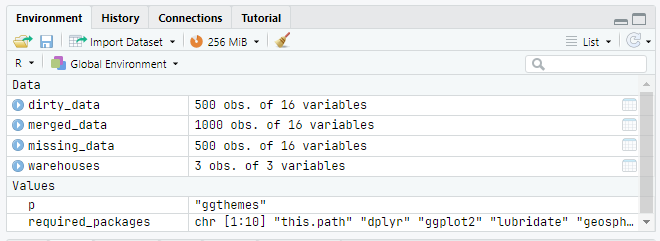
\includegraphics{Images/img/4.0_prepare_data/4.0_after_merge_files.PNG}
    \caption{Sau khi gộp 2 files CSV}
\end{figure}
\begin{boxH}
\textbf{Giải thích:} Thư viện \textbf{this.path} giúp tự động cập nhật đường dẫn thư mục gốc của dự án tại nơi chứa file R. Sau khi tải dữ liệu từ các file CSV mẫu, nhóm gộp hai file này thành một bảng duy nhất để thuận tiện xử lý.    
\end{boxH}
\subsection{Xác định Dữ liệu Khuyết}

Trong quá trình phân tích dữ liệu mẫu, nhóm đã tiến hành kiểm tra sự tồn tại của các giá trị bị khuyết (NA) trong bộ dữ liệu. Kết quả cho thấy một số cột có chứa giá trị khuyết, cụ thể như sau:

\begin{lstlisting}[language=r,caption={Các cột dữ liệu chứa giá trị bị khuyết}]
> na_cout<- colSums(is.na(merged_data ))
> print(na_cout)
                     order_id                   customer_id                          date 
                            0                             0                             0 
            nearest_warehouse                 shopping_cart                   order_price 
                           10                             0                            10 
             delivery_charges                  customer_lat                 customer_long 
                            0                            10                            10 
              coupon_discount                   order_total                        season 
                            0                            10                            10 
        is_expedited_delivery distance_to_nearest_warehouse        latest_customer_review 
                            0                            10                             0 
            is_happy_customer 
                           10 
\end{lstlisting}
\begin{boxH}
    Để phục vụ mục đích làm bài tập lớn và vẽ đồ thị, nhóm đã quyết định bỏ đi ba cột \textbf{distance\textunderscore{to}\textunderscore{nearest}\textunderscore{warehouse}} , \textbf{customer\textunderscore{long}} và \textbf{customer\textunderscore{lat}} và \textbf{nearst\textunderscore{warehouses}}.
\end{boxH}
\subsection{Làm sạch dữ liệu}
\subsubsection{Order\textunderscore{price}, Order\textunderscore{Total}}
Để xử lý các giá trị bị khuyết ở hai cột \textbf{order\_price} và \textbf{order\_total}, nhóm áp dụng công thức:

\begin{equation}
\textbf{order\_total} = \frac{\textbf{order\_price} \times (100 - \textbf{coupon\_discount})}{100} + \textbf{delivery\_charges}
\end{equation}
\noindent
\begin{equation}
\noindent
\textbf{order\_price} = \frac{(\textbf{order\_total} - \textbf{delivery\_charges}) \times 100}{100 - \textbf{coupon\_discount}}
\end{equation}



\begin{lstlisting}[language=R, caption=Xử lý cột \textbf{order\_total} và \textbf{order\_price}]
merged_data <- merged_data %>%
  mutate(
    order_total = ifelse(is.na(order_total), order_price * (100 - coupon_discount) / 100 + delivery_charges, order_total),
    order_price = ifelse(is.na(order_price), (order_total - delivery_charges) * 100 / (100 - coupon_discount), order_price)
  )

\end{lstlisting}
\textbf{Giải thích:} Hàm \textbf{mutate} của thư viện \textbf{dplyr} được sử dụng để thêm hoặc cập nhật cột trong bảng dữ liệu.

\subsubsection{season}

Ở cột \textbf{season}, nhóm nhận thấy một số giá trị không đồng nhất về cách viết hoa hoặc viết thường, dẫn đến dữ liệu thiếu đồng bộ được thể hiện dưới đây:

\begin{lstlisting}[language=R, caption=Giá trị cột \textbf{season} ban đầu]
season_unique_before<-unique(merged_data$season)
print(season_unique_before)

\end{lstlisting}

\begin{lstlisting}[language=R, caption=Xử lý cột \textbf{season}]
merged_data$season <- tolower(merged_data$season) # Đổi tất cả giá trị mùa dạng viết thường
month_value <- month(merged_data$date) # lấy tháng trong cột $date
merged_data <- merged_data %>%
  # Toán tử %>% : Truyền kết quả của phép toán hoặc hàm vào hàm tiếp theo .
  # mutate: Tạo ra cột mới hoặc thay đổi giá trị các cột trong data frame
  mutate(season = case_when(
    !is.na(season) ~ season,
    month_value %in% c(12, 1, 2) ~ "winter",
    month_value %in% c(3, 4, 5) ~ "spring",
    month_value %in% c(6, 7, 8) ~ "summer",
    TRUE ~ "autumn"
  ))

\end{lstlisting}
\begin{boxH}
\textbf{Giải thích:} Nhóm đã lấy giá trị \textbf{tháng} trong cột \textbf{date} của dữ liệu mẫu và sử dụng hàm \textbf{case\textunderscore{when}} xuất ra mùa và thế vào các giá trị bị khuyết. 
\end{boxH}
\begin{lstlisting}[language=R, caption=Dữ liệu cột \textbf{season} sau khi xử lý]
> season_unique_after<-unique(merged_data$season)
> print(season_unique_after)
[1] "winter" "summer" "autumn" "spring"
\end{lstlisting}

\subsubsection{is\textunderscore{happy}\textunderscore{customer}}
\begin{lstlisting}[language=R, caption=Làm tròn trung vị]
median_happy_customer <- round(median(merged_data$is_happy_customer, na.rm = TRUE), digits = 0)
merged_data$is_happy_customer[is.na(merged_data$is_happy_customer)] <- median_happy_customer
\end{lstlisting}
\begin{boxH} 
\textbf{Giải thích:}
    Lí do nhóm sử dụng giá trị trung vị cho cột 
is\textunderscore{happy}\textunderscore{customer} để \textbf{phản ánh độ hài lòng của khách hàng}, chúng chỉ có rơi vào một trong hai trường hợp là 0 và 1 (Hài lòng hoặc không hài lòng) và không ảnh hưởng bởi các giá trị ngoại lai .
\end{boxH}
\subsubsection{Kiểm tra dữ liệu sau khi làm sạch}
Sau khi dữ liệu được làm sạch, kiểm tra có cột nào còn dính giá trị bị khuyết nữa không.

\begin{lstlisting}[language=R, caption=Kiểm tra dữ liệu bị khuyết sau khi làm sạch]
> na_cout<- colSums(is.na(merged_data ))
> print(na_cout)
                     order_id                   customer_id                          date 
                            0                             0                             0 
            nearest_warehouse                 shopping_cart                   order_price 
                           10                             0                             0 
             delivery_charges                  customer_lat                 customer_long 
                            0                            10                            10 
              coupon_discount                   order_total                        season 
                            0                             0                             0 
        is_expedited_delivery distance_to_nearest_warehouse        latest_customer_review 
                            0                            10                             0 
            is_happy_customer 
                            0 
> 
\end{lstlisting}

% Xong phần làm sạch dữ liệu
\section{Mô Tả Thống Kê}
\subsection{Xử lý các điểm Outlier}
Sau khi xử lý dữ liệu gốc, nhóm phát hiện rằng một số cột trong bộ dữ liệu xuất hiện những điểm bất thường, dẫn đến sai lệch nghiêm trọng. Điều này có thể bắt nguồn từ lỗi trong bộ dữ liệu gốc hoặc phát sinh trong quá trình xử lý. Những giá trị này được nhận diện là outliers.
Để xác định các cột chứa giá trị ngoại lai, nhóm sử dụng \textit{Boxplot} để trực quan hóa dữ liệu.
\begin{lstlisting}[language=R, caption=Phát hiện giá trị outlier]
ggplot(data = merged_data, aes(y = order_price)) +
  geom_boxplot(outlier.shape = 16, outlier.colour = "red", outlier.fill = "red") +
  theme_minimal() +
  labs(
    title = "Điểm ngoại lai của order_price",
    y = ""
  )
ggplot(data = merged_data, aes(y = order_total)) +
  geom_boxplot(outlier.shape = 16, outlier.colour = "red", outlier.fill = "red") +
  theme_minimal() +
  labs(
    title = "Điểm ngoại lai của order_total",
    y = ""
  )

\end{lstlisting}

\begin{figure}[!ht]
    \centering 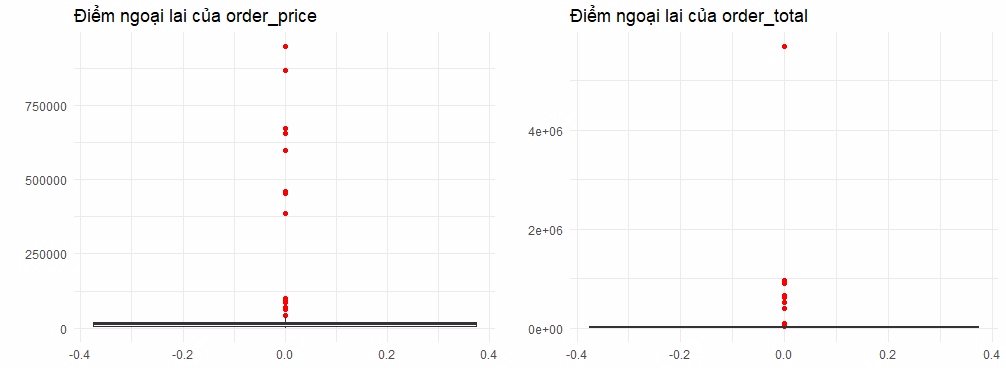
\includegraphics[width=15cm]{Images/img/4.2_remove_outlier/ngoai_loai_order_total_order_price.jpg}
    \caption{Điểm ngoại lai được đánh dấu đỏ}
\end{figure}

Qua phân tích, các cột được phát hiện có chứa outliers bao gồm:
\begin{itemize}
    \item \texttt{order\_price}
    \item \texttt{order\_total}
\end{itemize}
Để loại bỏ điểm ngoại lai này, nhóm áp dụng phương pháp tính Độ trải giữa (\textit{Interquartile Range}, viết tắt là IQR). Cụ thể, nhóm đặt cận trên \textit{Whisker Upper} và \textit{cận dưới} theo công thức sau:

\begin{itemize}
    \item \textbf{Cận trên} 
    $$( Q3 + 1.5) \times \text{IQR (độ trải giữa)}$$
    \item \textbf{Cận dưới} 
    $$( Q1 - 1.5) \times \text{IQR (độ trải giữa)}$$
\end{itemize}
Những giá trị vượt qua cận trên hoặc dưới sẽ được thay thế bằng chính giá trị tương ứng của những cận này.

\begin{lstlisting}[language=R, caption=Xử lý giá trị ngoại lai bằng phương pháp IQR]
# Tính toán các tứ phân vị cho các cột order_price và order_total
quantiles_price <- quantile(merged_data$order_price)
quantiles_total <- quantile(merged_data$order_total)
# Trong R , hàm quanlite trả về 5 giá trị cùng [index]
# [1]: 0%
# [2]: 25% [Q1]
# [3]: 50%
# [4]: 75% [Q3]
# [5]: 100%
# Hàm tứ phân vị trong R
q1_price <- quantiles_price[2]
q3_price <- quantiles_price[4]
q1_total <- quantiles_total[2]
q3_total <- quantiles_total[4]
# Tính IQR cho order_price và order_total
IQR_price <- q3_price - q1_price
IQR_total <- q3_total - q1_total

# Hàm tính giá trị biên dưới (lower) và biên trên (upper) của IQR
calc_lower <- function(Q1, IQR) { return(Q1 - 1.5 * IQR) }
calc_upper <- function(Q3, IQR) { return(Q3 + 1.5 * IQR) }

# Tính giá trị cận dưới và cận trên cho order_price và order_total
lower_price <- calc_lower(q1_price, IQR_price)
upper_price <- calc_upper(q3_price, IQR_price)
lower_total <- calc_lower(q1_total, IQR_total)
upper_total <- calc_upper(q3_total, IQR_total)
# Điều chỉnh giá trị order_total ra ngoài phạm vi IQR
for (i in 1:length(merged_data$order_total)) {
  Tạo một vòng lặp cho cột order_total
  if (merged_data$order_total[i] > upper_total) {
    merged_data$order_total[i] = upper_total  # Thay giá trị cận trên của order_total
  } else if(merged_data$order_total[i] < lower_total ){
    merged_data$order_total[i] = lower_total  # Thay giá trị cận dưới của order_total
  }
}
# Điều chỉnh giá trị order_price ra ngoài phạm vi IQR
## Tạo một vòng lặp cho cột order_price
for (i in 1:length(merged_data$order_price)) {
  if (merged_data$order_price[i] > upper_price) {
    merged_data$order_price[i] = upper_price  # Thay giá trị cận trên của order_price
  } else if(merged_data$order_price[i] < lower_price){
    merged_data$order_price[i] = lower_price  # Thay giá trị dưới của order_price
  }
}
\end{lstlisting}

\begin{figure}[!ht]
    \centering 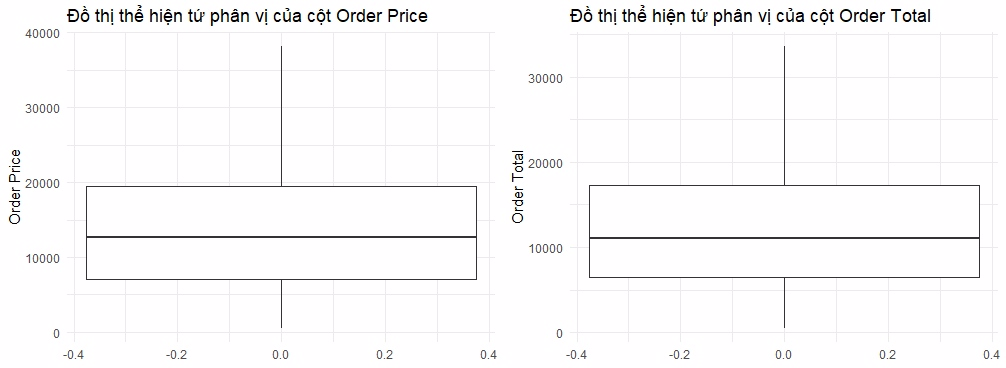
\includegraphics[width=15cm]{Images/img/4.2_remove_outlier/tu_phan_vi.jpg}
    \caption{Sau khi dùng tứ phân vị}
\end{figure}
\subsection{Thống kê dữ liệu}
Mục tiêu của nhóm là hiểu rõ hơn về chi phí và doanh thu trong từng mùa, từ đó đưa ra các quyết định hợp lý như thay đổi chiến lược giao hàng hoặc cải thiện hiệu quả kinh doanh trong các mùa. Hướng đến mục tiêu chung là cung cấp dịch vụ tốt nhất cho khách hàng theo từng thời điểm trong năm, nhóm đã thực hiện các phân tích thống kê về những hạng mục quan trọng bao gồm:

\begin{itemize}
    \item Kiểm tra sự tương quan giữa order\textunderscore{price} và order\textunderscore{total} 
    \item Tổng số đơn hàng theo từng mùa.
    \item Tổng chi phí giao hàng.
    
\end{itemize}

\begin{lstlisting}[language=R, caption=Thống kê]
season_summary <- merged_data %>%
  group_by(season) %>%
  summarise(
    total_orders = n(),
    avg_order_total = mean(order_total, na.rm = TRUE),
    total_delivery_charges = sum(delivery_charges, na.rm = TRUE)
  )
print(season_summary)

\end{lstlisting}
\begin{lstlisting}[language=R, caption=Thông số từng hạng mục theo mùa]
> print(season_summary)
  season total_orders avg_order_total total_delivery_charges
  <chr>         <int>           <dbl>                  <dbl>
1 autumn          247          12992.                 17277.
2 spring          266          12320.                 23526.
3 summer          249          12487.                 19892.
4 winter          238          12009.                 16475.
\end{lstlisting}
\subsubsection{Ma trận tương quan giữa order\textunderscore{price} và total\textunderscore{order}}
Trước khi vẽ đồ thị, nhóm muốn kiểm tra liệu có mối quan hệ giữa order\textunderscore{total} và order\textunderscore{price} hay không? Nhóm chọn phương pháp ma trận \textbf{cor} để thể hiện độ tương quan

\begin{lstlisting}[language=R,caption=Code kiểm tra độ tương quan]
overview_data <- merged_data[c("order_price", "delivery_charges", "coupon_discount","order_total", "is_expedited_delivery", "is_happy_customer", "shopping_cart")]
numeric_data <- overview_data[sapply(overview_data, is.numeric)]
cor_matrix <- cor(numeric_data)
# Hiện thi ma trận
corrplot(
  cor_matrix,
  method = "color",
  col= colorRampPalette(c("white","#202020", "#202040"))(10) ,
  type = "full",
  order = "hclust",
  tl.col = "black",
  tl.srt = 45,
  addCoef.col = "white",
  number.cex = 0.8,
  tl.cex = 0.8,
  diag = TRUE,
  cl.pos = "r"
)
\end{lstlisting}
% Ảnh
\begin{figure}[H]
    \centering 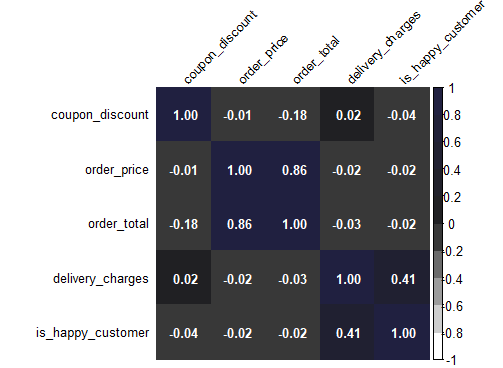
\includegraphics[width=15cm]{Images/img/4.3_plotting_data/order_price_total.png}
    \caption{Biểu đồ colorgram}
\end{figure}

\begin{boxH}
\textbf{Nhận xét:} Có sự tương quan giữa order\textunderscore{total} và order\textunderscore{price}.
\end{boxH}
% Đồ thị số
\subsubsection{Tổng đơn hàng theo mùa}
\begin{lstlisting}[language=R, caption=Đồ thị thể hiện tổng số đơn hàng theo từng mùa]
ggplot(data = season_summary, aes(x = season, y = total_orders, fill = season)) +
  geom_bar(stat = "identity") +
  geom_text(aes(label = total_orders), vjust = 2,color = "white", ) +
  theme_minimal() +
  labs(
    title = "Tổng số đơn hàng trong từng mùa",
    x = " ",
    y = " " # Để trống
  ) +
  scale_fill_brewer(palette = "Paired")
\end{lstlisting}

\begin{figure}[!ht]
    \centering 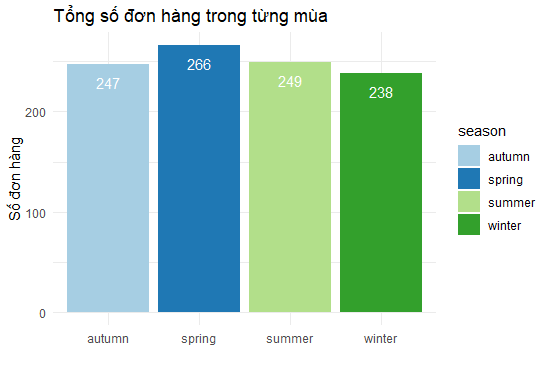
\includegraphics[width=15cm]{Images/img/4.3_plotting_data/1-total_order.png}
    \caption{Tổng số đơn hàng theo từng mùa}
    
\end{figure}
\begin{boxH}
\textbf{Nhận xét:} Vào mùa xuân (spring), khách hàng thường mua sắm nhiều hơn nên tổng số đơn hàng tập trung nhiều vào mùa xuân. Nhưng sự chênh lệch không đáng kể.
\end{boxH}
\subsubsection{Tổng phí giao hàng theo từng mùa}
\begin{lstlisting}[language=R, caption=Đồ thị Tổng chi phí giao hàng theo từng mùa]
ggplot(data = season_summary, aes(x = season, y = total_delivery_charges, fill = season)) +
  geom_bar(stat = "identity") +
  geom_text(aes(label = total_delivery_charges), vjust = 2,color = "white", ) +
  theme_minimal() +
  labs(
    title = "Tổng phí giao hàng từng mùa",
    x = " ",
    y = " " #Để trống
  ) +
  scale_fill_brewer(palette = "Set2")

\end{lstlisting}

\begin{figure}[!ht]
    \centering 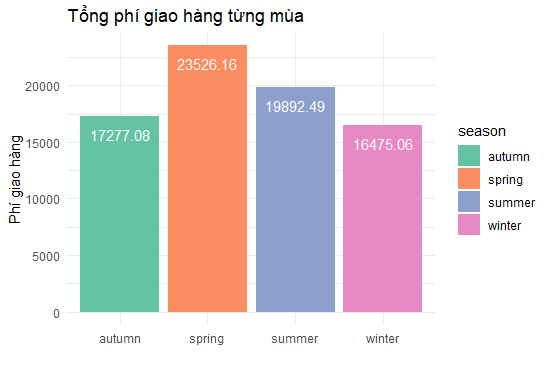
\includegraphics[width=15cm]{Images/img/4.3_plotting_data/2-delivery_charge.png}
    \caption{Tổng phí đơn hàng theo từng mùa}
\end{figure}
\textbf{Nhận xét:} Lượng chi phí đơn hàng đạt giá trị cao nhất vào mùa xuân và chúng nó độ chênh lệch cao giữa các mùa.

\textbf{Tổng kết:} Việc phân tích các chỉ số trên sẽ giúp nhóm có cái nhìn tổng quan và đưa ra các chiến lược phù hợp nhằm tối ưu hóa các yếu tố kinh doanh theo từng mùa, đáp ứng nhu cầu của khách hàng một cách tối đa.


\section{Thống Kê Suy Diễn}
\subsection*{Kiểm tra phân phối chuẩn}
Trước khi lựa chọn các phương pháp thống kê, nhóm phải kiểm tra dữ liệu \textbf{season}, price\textunderscore{total}, order\textunderscore{total}. có tuân theo bảng phân phối chuẩn hay không với phương pháp \textbf{shapiro}.
\begin{lstlisting}[language=R, caption=Shapiro Test]
# Trích xuất các cột order_price và order_total từ merged_data
get_order_price <- merged_data$order_price
get_order_total <- merged_data$order_total

# Kiểm tra phân phối chuẩn với Shapiro-Wilk cho cột order_total
shapiro_order_total <- shapiro.test(get_order_total)
# Kiểm tra phân phối chuẩn với Shapiro-Wilk cho cột order_price
shapiro_order_price <- shapiro.test(get_order_price)

# In kết quả kiểm tra Shapiro-Wilk cho toàn bộ dữ liệu
print(shapiro_order_price)  # Kết quả kiểm tra cho order_price
print(shapiro_order_total)  # Kết quả kiểm tra cho order_total
# Kiểm tra phân phối chuẩn theo từng mùa
seasons <- c("spring", "summer", "fall", "winter")
# Tạo danh sách để lưu giá trị order_price theo từng mùa
order_price_by_season <- list()
# Lặp qua từng mùa, trích xuất dữ liệu và lưu vào danh sách
for (season in seasons) {
  # Trích xuất dữ liệu của từng mùa bằng subset()
  season_data <- subset(merged_data, season == season)  
  # Lưu giá trị order_price của từng mùa vào danh sách
  order_price_by_season[[season]] <- season_data$order_price
}
# Tạo bảng tóm tắt kết quả kiểm tra Shapiro-Wilk cho từng mùa
shapiro_summary <- data.frame(
  Season = names(order_price_by_season),  # Tên các mùa
  P_value = sapply(order_price_by_season, function(order_price) {
    # Tính p-value từ kiểm tra Shapiro-Wilk cho từng mùa
    shapiro.test(order_price)$p.value
  })
)
# Đánh giá phân phối chuẩn: nếu p-value > 0.05 thì phân phối chuẩn
shapiro_summary$Normal_Distribution <- ifelse(shapiro_summary$P_value > 0.05, "True",  # Phân phối chuẩn
"False") # Không phải phân phối chuẩn
# In bảng tóm tắt kết quả kiểm tra Shapiro-Wilk theo mùa
print(shapiro_summary)

\end{lstlisting}
\begin{table}[H]
\centering
\begin{tabular}{|l|r|c|} % Cột: l (trái), r (phải), c (giữa)
\hline
\textbf{Mùa} & \textbf{P-value}       & \textbf{Có phải phân phối chuẩn?} \\ \hline
spring          & 7.348016e-18          & Không                        \\ \hline
summer          & 7.348016e-18          & Không                        \\ \hline
fall            & 7.348016e-18          & Không                        \\ \hline
winter          & 7.348016e-18          & Không                        \\ \hline
\end{tabular}
\caption{Kiểm tra phân phối chuẩn của mùa}
\label{tab:normality_results}
\end{table}
\begin{lstlisting}[language=R,caption=Hai cột còn lại]
> print(shapiro_order_price)  # Kết quả kiểm tra cho order_price
	Shapiro-Wilk normality test
data:  get_order_price
W = 0.95034, p-value < 2.2e-16
> print(shapiro_order_total)  # Kết quả kiểm tra cho order_total
	Shapiro-Wilk normality test
data:  get_order_total
W = 0.94557, p-value < 2.2e-16

% Giới thiệu

\end{lstlisting}
\begin{boxH}
    \textbf{Nhận xét:} Từ những dữ kiện trên, ta có thể kết luận chúng không tuân theo phân phối chuẩn.
\end{boxH}
\subsection{Kiểm định trung bình một mẫu}
\subsubsection{Bài toán thực tế}
Để kiểm định giá trị trung bình một mẫu, nhóm đã đặt giả thuyết rằng doanh thu bán hàng của cửa hàng trong mùa Xuân có bằng với doanh thu kì vọng là 50 triệu đồng hay không? ($\mu$ = $50$)  
Nhóm đưa ra hai giả thuyết như sau:

\textbf{Giả thuyết kiểm định:}
\begin{itemize}
    \item \( H_0 \): \( \mu = 50 \) 
    \item \( H_1 \): \( \mu > 50 \) 
\end{itemize}

\subsubsection{Mô tả dữ liệu và công thức tính}

\begin{lstlisting}[language=R, caption=Tính các thông số]
spring_data <- merged_data %>%
  filter(season == "spring")
## Xuất ra trung bình mẫu, sd , muy
spring_stats <- spring_data %>%
  summarise(
    mean = mean(order_total),
    sd = sd(order_total),
    n = n()
  )  
\end{lstlisting}

\begin{table}[h!]
\centering
\begin{tabular}{|l|r|}
\hline
\textbf{Thông số} & \textbf{Giá trị} \\
\hline
Trung bình mẫu \( \bar{X} \) & 12,320 \\
Giá trị kỳ vọng \( \mu_0 \) & 50 \\
Độ lệch chuẩn mẫu \( s \) & 7,757 \\
Số quan sát \( n \) & 266 (vì df = 265) \\
\hline
\end{tabular}
\caption{Các thông số thống kê dùng trong bài toán kiểm định một mẫu}
\label{tab:thongso}
\end{table}

Áp dụng công thức lý thuyết cho trường hợp phân phối tuỳ ý, mẫu $\geq$ $30$ ,  ta có công thức tính giá trị kiểm định như sau:
\begin{boxH}
\[
Z_{qs} = \frac{\bar{X} - \mu_0}{\dfrac{s}{\sqrt{n}}}
\]

\textbf{Thay số vào:}

\[
Z = \frac{12320 - 50}{\dfrac{7757}{\sqrt{266}}}
= \frac{12270}{474.89} \approx 25.83
\]
\end{boxH}

\subsubsection{Xử lý trên phần mềm RStudio}
Xử lý trên phần mềm RStudio, nhóm sử dụng hàm \texttt{z.test} để tính giá trị kiểm định và p-value. Cụ thể, nhóm sử dụng hàm này với các tham số như sau:

\begin{lstlisting}[language=R, caption=Kiểm định một mẫu]
z.test(x = spring_data$order_total,
       mu = 50,
       sigma.x = sd(spring_data$order_total),
       alternative = "greater")
\end{lstlisting}


\subsubsection{Kết luận}

\begin{lstlisting}[language=R, caption=Kết quả sau khi dùng t-test]
    One-sample z-Test
data:  spring_data$order_price
z = 28.704, p-value < 2.2e-16
alternative hypothesis: true mean is greater than 50
95 percent confidence interval:
 12920.34       NA
sample estimates:
mean of x 
 13702.69 
\end{lstlisting}

\begin{boxH}
    Kết luận: p-value < 0.05, như vậy ta có thể khẳng định , không đủ điều kiện để bác bỏ $H_0$
\end{boxH}


% Ý tưởng hai mẫu (t-test)
\subsection{Kiểm định trung bình hai mẫu}
\subsubsection{Bài toán thực tế}
Sau khi đã xác định được doanh thu của cửa hàng tại mùa xuân không vượt qua giá trị kì vọng, nhóm tiếp tục đem so sánh dữ liệu \textbf{mùa xuân}
so với \textbf{mùa hè} với mức ý nghĩa $\alpha$ = 0.05

Nhóm đặt giả thuyết như sau
\begin{itemize}
    \item \textbf{Giả thuyết không (H\textsubscript{0}):} $\mu_1 = \mu_2$ 
    \item \textbf{Giả thuyết đối (H\textsubscript{1}):} $\mu_1 \ne \mu_2$ 
\end{itemize}
\subsubsection{Tính giá trị kiểm định}
Để tính giá trị kiểm định, nhóm sử dụng phương pháp tách 2 mẫu \textbf{xuân} và \textbf{hè} ra làm 2 và lọc ra thông số độ lệch chuẩn, n (số mẫu) và mean (trung bình mẫu)

\begin{lstlisting}[language=R, caption=Chia nhóm và tính toán chỉ số đặc trưng ]
group_stats <- merged_data %>%
  filter(season %in% c("spring", "summer")) %>%
  group_by(season) %>%
  summarise(
    mean = mean(order_total),
    sd = sd(order_total),
    n = n(),
    .groups = "drop"
  )
print(group_stats)

\end{lstlisting}
\subsubsection{Mô tả dữ liệu và công thức tính}
\begin{table}[H]
\centering
\caption{ Chỉ số bài toán \texttt{order\_total} theo mùa Xuân và Hè}
\begin{tabular}{@{}lccc@{}}
\textbf{Mùa} & \textbf{Trung bình (\textmu)} & \textbf{Độ lệch chuẩn (s)} & \textbf{Số lượng (n)} \\
Xuân (Spring) & 12,320 & 7,757 & 266 \\
Hè (Summer)   & 12,487 & 7,697 & 249 \\
\end{tabular}
\end{table}
Công thức tính cho trường hợp kiểm định 2 mẫu độc lập, có phân phối tuỳ ý và 2 mẫu $\geq$ $30$ như sau:
\[
Z_{qs} = \frac{\overline{X}_1 - \overline{X}_2}
{\sqrt{\frac{s_1^2}{n_1} + \frac{s_2^2}{n_2}}}
\]
\begin{boxH}

Thế số vào:
\[
Z = \frac{12319.55 - 12486.75}{\sqrt{\frac{7757.41^2}{266} + \frac{7697.42^2}{249}}} \approx -0.24542
\]
  
\end{boxH}
\subsubsection{Xử lý trên phần mềm RStudio}
Xử lý trên phần mềm RStudio, nhóm sử dụng hàm \texttt{t.test} để tính giá trị kiểm định và p-value. Cụ thể, nhóm sử dụng hàm này với các tham số như sau:
\begin{lstlisting}[language=R, caption=Các thông số thống kê dùng trong kiểm định trung bình 2 mẫu ]
  t_test_result_two_sample<-t.test(order_total ~ season, 
       data = merged_data %>% filter(season %in% c("spring", "summer")),
       var.equal = FALSE) # giả định phương sai không bằng nhau
print(t_test_result_two_sample)
\end{lstlisting}

\begin{lstlisting}[language=R, caption= Kết quả t-test]
		Welch Two Sample t-test

data:  order_total by season
t = -0.24542, df = 511.26, p-value = 0.8062
alternative hypothesis: true difference in means between group spring and group summer is not equal to 0
95 percent confidence interval:
 -1505.705  1171.298
sample estimates:
mean in group spring mean in group summer 
            12319.55             12486.75 
\end{lstlisting}

\subsubsection{Kết luận}
\begin{boxH}

Với $p_value = 0.8602 > 0.05$ , nhóm không có đủ bằng chứng để bác bỏ giả thuyết $H_0$ tức là không có sự khác biệt trong doanh thu giữa hai mùa.

\end{boxH}
% Anova
\subsection{Anova một yếu tố}

\subsubsection{Bài toán thực tế}
Một cửa hàng điện tử muốn kiểm tra xem \textbf{giá trị đơn hàng trung bình} (\texttt{order\_total}), với cỡ mẫu của mỗi nhóm là $30$, có bị ảnh hưởng bởi \textbf{mùa vụ} (\texttt{season}) hay không.  
Dữ liệu được thu thập từ các đơn hàng, phân loại thành $4$ nhóm theo mùa: \textbf{Winter} (mùa đông), \textbf{Summer} (mùa hè), \textbf{Autumn} (mùa thu) và \textbf{Spring} (mùa xuân).  

Với mức ý nghĩa $\alpha = 5\%$, sử dụng phương ph \textbf{mô hình ANOVA một yếu tố} để kiểm tra xem giá trị đơn hàng trung bình giữa các mùa có sự khác biệt đáng kể hay không.
\subsubsection{Giả thuyết kiểm định}

\begin{itemize}
  \item Các tổng thể phải tuân theo phân phối chuẩn $N(\mu, \sigma^2)$
  \item Số nhóm $k=4$
  \item Phương sai bằng nhau $\sigma_1^2 = \sigma_2^2 = \sigma_3^2 = \sigma_4^2$
  \item Các mẫu quan sát (từ $k$ tổng thể) được lấy độc lập, với $n = 30$ cho mỗi nhóm, tổng số quan sát $N = 120$.
  \item 
\end{itemize}

\subsubsection{Hiện thực phép toán}
Gọi $\mu_i$ là giá trị đơn hàng trung bình của mùa thứ $i$.
\begin{align*}
    H_0 &: \mu_1 = \mu_2 = \mu_3 = \mu_4, \\
    % H_1 &: \exists\ i \neq j \ \text{sao cho} \ \mu_i \neq \mu_j.
    H_1 &: \exists\ \mu_i \neq \mu_j \ \text{sao cho} \ i \neq j.
\end{align*}

\subsubsection{Tính các tham số mẫu}
\begin{table}[H]
\centering
\caption{Trung bình và phương sai mẫu theo mùa}
\begin{tabular}{lcc}
\hline
Mùa & Trung bình mẫu $\overline{x}_i$ & Phương sai mẫu $s_i^2$ \\ \hline
Winter  & $12499.31$ & $56,686,589.91$ \\
Summer  & $12493.37$ & $61,622,987.35$ \\
Autumn  & $12858.15$ & $48,321,908.37$ \\
Spring  & $14594.52$ & $106,019,827.40$ \\ \hline
\end{tabular}
\end{table}
Trung bình tổng thể \textbf{$\overline{x}$} là $1311.33$
\subsubsection{Giá trị trong và giữa các nhóm}

\paragraph{Tổng bình phương giữa nhóm (SSB):}
\[
SSB = 14,303,293.20 + 14,550,442.35 + 3,299,751.675 + 55,465,154.35 = 87,618,641.575
\]
Bình phương trung bình giữa nhóm (MSB):
\[
MSB = \frac{SSB}{k-1} = \frac{87,618,641.575}{3} \approx 29,206,213.86
\]

\paragraph{Tổng bình phương trong nhóm (SSW):}
\[
SSW = 1,643,911,107 + 1,787,066,635 + 1,401,335,343 + 3,074,574,995 = 7,906,888,080
\]
Bình phương trung bình trong nhóm (MSW):
\[
MSW = \frac{SSW}{N-k} = \frac{7,906,888,080}{116} \approx 68,162,828.28
\]

\subsubsection{Giá trị thống kê kiểm định}
\[
F = \frac{MSB}{MSW} = \frac{29,206,213.86}{68,162,828.28} \approx 0.4285
\]

\subsubsection{Miền bác bỏ}
Với $\alpha = 5\%$, $df_1 = k-1 = 3$, $df_2 = N-k = 116$:
\[
F_{0.05; 3; 116} \approx 2.6802
\]
Miền bác bỏ:
\[
RR = (2.6802, +\infty)
\]

\subsubsection{Kết luận}
\begin{boxH}

\textbf{Kết luận:} 
Vì $F \approx 0.4285 < 2.6802$, không bác bỏ $H_0$ nên không có bằng chứng thống kê cho thấy giá trị đơn hàng trung bình giữa các mùa khác biệt đáng kể.

\end{boxH}

\subsection{Xử lý trên phần mềm R}
Sử dụng phương pháp leveneTest trong R để thực hiện
\begin{lstlisting}[language=R, caption=Phép kiểm ANOVA một yếu tố]
df_cleaned <- merged_data %>%
  group_by(season) %>%
  mutate(order_total_cleaned = ifelse(order_total > quantile(order_total, 0.75) + 1.5 * IQR(order_total) | order_total < quantile(order_total, 0.25) - 1.5 * IQR(order_total), NA, order_total)) %>%
  ungroup()
leveneTest(order_total_cleaned ~ season, data = df_cleaned)
anova_model <- aov(order_total_cleaned ~ season, data = df_cleaned)
summary(anova_model)
\end{lstlisting}

\begin{lstlisting}[language=R, caption=Kết quả ANOVA một yếu tố]
Df    Sum Sq   Mean Sq F value Pr(>F)  
season        3 3.576e+08 119214928   2.299 0.0759 .
Residuals   981 5.086e+10  51848700 
  
\end{lstlisting}
Kết luận: Không đủ điều kiện để bác bỏ giả thuyết $H_0$ với $p$-value = 0.0759 > 0.05, tức là không có sự khác biệt đáng kể giữa giá trị đơn hàng trung bình của các mùa.
\subsection{Hồi quy tuyến tính}

\subsubsection{Bài toán thực tế}
Xây dựng mô hình hồi quy tuyến tính với biến phụ thuộc:
\[
Y = \texttt{order\_price}
\]
và hai biến độc lập:
\[
X_1 = \texttt{coupon\_discounts}, \quad X_2 = \texttt{delivery\_charges}.
\]
Mô hình hồi quy bội được viết dưới dạng:
\[
Y = \beta_0 + \beta_1 X_1 + \beta_2 X_2 + \varepsilon_i, \quad i = 1, 2, \ldots, n
\]
trong đó:
\begin{itemize}
    \item $Y$: Giá trị đơn hàng (\texttt{order\_price})
    \item $X_1$: Giảm giá bằng coupon (\texttt{coupon\_discounts})
    \item $X_2$: Phí giao hàng (\texttt{delivery\_charges})
    \item $\varepsilon_i$: Sai số ngẫu nhiên, có kỳ vọng $E(\varepsilon) = 0$, phương sai $\sigma^2$
\end{itemize}

\subsubsection{Cơ sở lý thuyết}
Mô hình hồi quy bội mở rộng mô hình hồi quy đơn bằng cách đưa vào nhiều biến độc lập:
\[
Y = \beta_0 + \beta_1 X_1 + \beta_2 X_2 + \dots + \beta_p X_p + \varepsilon
\]
\begin{itemize}
    \item $\beta_0$: Hệ số chặn
    \item $\beta_j$: Hệ số hồi quy của biến độc lập $X_j$
    \item $\varepsilon$: Sai số ngẫu nhiên
\end{itemize}

\subsubsection{Phương pháp ước lượng}
Sử dụng phương pháp \textbf{Bình phương tối thiểu (OLS)}:
\[
\hat{\beta} = (X^\mathsf{T}X)^{-1} X^\mathsf{T} Y
\]
trong đó:
\begin{itemize}
    \item $X$: Ma trận giá trị các biến độc lập $(n \times (p+1))$
    \item $Y$: Vector giá trị của biến phụ thuộc $(n \times 1)$
    \item $\hat{\beta}$: Vector hệ số hồi quy $(p+1) \times 1$
\end{itemize}

\paragraph{Hệ số xác định $R^2$:}
\[
R^2 = 1 - \frac{SS_\text{res}}{SS_\text{tot}}
\]
với:
\[
SS_\text{res} = \sum_{i=1}^n (y_i - \hat{y}_i)^2, \quad SS_\text{tot} = \sum_{i=1}^n (y_i - \overline{y})^2
\]

\subsubsection{Kết quả mô hình OLS}
Mô hình trong R:
\begin{verbatim}
model <- lm(order_price ~ coupon_discount + delivery_charges, data = df)
summary(model)
\end{verbatim}

\paragraph{Kiểm tra đa cộng tuyến:}
\begin{verbatim}
vif(model)
# coupon_discount: 1.000546
# delivery_charges: 1.000546
\end{verbatim}
$\Rightarrow$ VIF xấp xỉ 1 cho cả hai biến, không xảy ra đa cộng tuyến.

\paragraph{Hệ số ước lượng:}
\[
\hat{\beta}_0 = 13297.85, \quad \hat{\beta}_1 = 143.66, \quad \hat{\beta}_2 = 59.37
\]
Ý nghĩa:
\begin{itemize}
    \item Khi $X_1$ tăng 1 đơn vị, $Y$ tăng trung bình $143.66$
    \item Khi $X_2$ tăng 1 đơn vị, $Y$ tăng trung bình $59.37$
\end{itemize}

\paragraph{Kiểm định $t$:}
\begin{itemize}
    \item $X_1$: $p = 0.527 > 0.05$ $\Rightarrow$ không đủ bằng chứng biến có ý nghĩa
    \item $X_2$: $p = 0.662 > 0.05$ $\Rightarrow$ không đủ bằng chứng biến có ý nghĩa
\end{itemize}

\paragraph{Kiểm định $F$:}
$p$-value lớn hơn 0.05, $R^2 \approx 0$ $\Rightarrow$ mô hình không có ý nghĩa thống kê, biến phụ thuộc quan hệ yếu với các biến độc lập.
% Update 5/12/2024
\vfil\penalty-200\vfilneg
\section{Thảo luận và Mở rộng}

\subsection{Nhận xét dữ liệu}
\begin{itemize}
    \item  Trong mô hình tổng quan, có những cột dữ liệu không tuân theo phân phối chuẩn như \textbf{order\_total} và \textbf{order\_price}. Điều này có thể do sự hiện diện của các giá trị ngoại lai hoặc phân phối không đồng nhất.
    \item Phương sai không đồng nhất , có thể do sự biến động lớn trong giá trị đơn hàng giữa các mùa. 
    \item Có những cột phụ thuộc với nhau, ví dụ \textbf{order\_price} ảnh hưởng bởi \textbf{coupon\_discount}.

\end{itemize}

\subsection{Tính bao quát}

Nhóm đã phân tích các yếu tố ảnh những ảnh hưởng đến sự thay đổi của dữ liệu, cũng như phân tích và kiểm định trong từng trường hợp như sau:
Các kiểm định được chọn phù hợp với mục tiêu và đặc điểm dữ liệu (không chuẩn, không đồng nhất phương sai, có cặp). Ngoài ra, nhóm cũng mở rộng bằng kiểm định hậu nghiệm (Dunn Test) để phân tích sâu hơn sau Kruskal-Wallis. Do đó, phân tích được đánh giá là có tính bao quát tốt và hợp lý về mặt phương pháp.
Cụ thể các phương pháp đã được nhóm sử dụng như sau: 
\begin{itemize}
    \item Phân tích 1 mẫu với \textbf{z-test}
    \item Phân tích 2 mẫu với \textbf{t-test}
    \item Phân tích Annova \textbf bằng {Krustal-Wallis}
    \item Phân tích hồi quy tuyến tính
\end{itemize}
\subsection{Điểm mạnh và điểm yếu của các phương pháp đã sử dụng}

\begin{table}[H]
\centering
\caption{Tổng hợp ưu điểm và nhược điểm của các phương pháp kiểm định}
\label{tab:summary_tests}
\renewcommand{\arraystretch}{1} % Giãn dòng trong bảng
\begin{tabular}{|p{3.2cm}|p{5.5cm}|p{5.5cm}|}
    
\hline
\textbf{Phương pháp} & \textbf{Ưu điểm} & \textbf{Nhược điểm} \\ \hline
% 1 mẫu
\textbf{Z-test một mẫu} &
\begin{itemize}[leftmargin=*, topsep=0pt, partopsep=0pt, parsep=0pt, itemsep=0pt]
\item Dễ hiểu và triển khai.
    \item Hiệu quả với cỡ mẫu lớn (n > 30).
    \item Không yêu cầu phân phối chuẩn nhờ định lý giới hạn trung tâm.
\end{itemize} &
\begin{itemize}[leftmargin=*, topsep=0pt, partopsep=0pt, parsep=0pt, itemsep=0pt]
    \item Giả định dữ liệu độc lập, mẫu đại diện.
    \item Không phù hợp với cỡ mẫu nhỏ.
\end{itemize} \\ \hline
% 2 mẫu
\textbf{T-test hai mẫu (Welch)} &
\begin{itemize}[leftmargin=*, topsep=0pt, partopsep=0pt, parsep=0pt, itemsep=0pt]
    \item So sánh hai nhóm độc lập.
    \item Không yêu cầu phương sai bằng nhau.
\end{itemize} &
\begin{itemize}[leftmargin=*, topsep=0pt, partopsep=0pt, parsep=0pt, itemsep=0pt]
    \item Nhạy cảm với ngoại lai nếu dữ liệu không chuẩn.
    \item Cần số lượng mẫu đủ lớn nếu phân phối không chuẩn.
\end{itemize} \\ \hline
% Annova
\textbf{Anova 1 yếu tố}&
\begin{itemize}[leftmargin=*, topsep=0pt, partopsep=0pt, parsep=0pt, itemsep=0pt]
    \item  Dễ hiểu và thực hiện
    \item Có khả năng mở rộng hay kết hợp với các kiểm định bổ sung như Tukey's HSD để xác định cụ thể nhóm nào khác biệt.
\end{itemize} &
\begin{itemize}[leftmargin=*, topsep=0pt, partopsep=0pt, parsep=0pt, itemsep=0pt]
    \item Yêu cầu tổng thể có phân phối chuẩn.
    \item Không chỉ ra cặp nhóm nào khác biệt.
    \item Cần kiểm định hậu nghiệm (như Dunn Test).
\end{itemize} \\ \hline

% Hồi quy tuyến tính
\textbf{Phương pháp OLS trong hồi quy tuyến tính} &
\begin{itemize}[leftmargin=*, topsep=0pt, partopsep=0pt, parsep=0pt, itemsep=0pt]
    \item Dễ hiểu, tính toán nhanh, nhiều công cụ kiểm định, nền tảng lý thuyết vững
\end{itemize} &
\begin{itemize}[leftmargin=*, topsep=0pt, partopsep =0pt, parsep=0pt, itemsep=0pt]
    \item Nhạy cảm với ngoại lai, cần giả định chặt chẽ, không xử lý tốt dữ liệu phi tuyến, đa cộng tuyến làm mất ổn định
\end{itemize} \\ \hline 

\end{tabular}
\end{table}

\subsection{Mối quan hệ giữa mục tiêu và phương pháp được chọn}

Mục tiêu chính của nghiên cứu không phải là dự đoán giá trị, mà là kiểm tra xem các yếu tố như mùa vụ, đặc điểm sản phẩm hay hành vi mua hàng có tạo ra sự khác biệt có ý nghĩa thống kê về giá trị đơn hàng hay không. 

Nhóm lựa chọn các phương pháp sau:
\begin{enumerate}
    \item \textbf{Z-test một mẫu}: kiểm tra sự khác biệt giữa trung bình mẫu và giá trị giả thuyết.
    \item \textbf{T-test hai mẫu (Welch)}: so sánh trung bình của hai nhóm độc lập khi phương sai không đồng nhất.
    \item \textbf{ANOVA một yếu tố}: kiểm tra sự khác biệt trung bình giữa nhiều nhóm; nếu có ý nghĩa thống kê, mở rộng thêm \textbf{Dunn test} để xác định cặp nhóm khác biệt.
    \item \textbf{Hồi quy tuyến tính}: phân tích tác động của biến độc lập lên biến phụ thuộc và đánh giá mức độ giải thích của mô hình.
\end{enumerate}

Việc lựa chọn trên đảm bảo phù hợp với đặc điểm dữ liệu, đáp ứng mục tiêu so sánh sự khác biệt và phân tích mối quan hệ, thay vì thuần túy dự đoán.
\subsection{Mở rộng với phương pháp Kruskal-Wallis}
\begin{boxH}
    Nguyên lý của phương pháp Kruskal-Wallis
\begin{itemize}
    \item Sắp xếp tất cả các quan sát từ nhỏ đến lớn và gán thứ hạng (rank).
    \item Tính tổng thứ hạng cho từng nhóm.
    \item So sánh sự khác biệt tổng thứ hạng giữa các nhóm để đánh giá liệu các nhóm có xuất phát từ cùng một phân phối hay không.
\end{itemize}
\end{boxH}

Lí do nhóm chọn \textbf{Kruskal-Wallis} là vì:
\begin{itemize}
    \item Dữ liệu không tuân theo phân phối chuẩn và có phương sai không đồng nhất.
    \item Kruskal-Wallis là phương pháp phi tham số, không yêu cầu giả định phân phối chuẩn.
    \item Phù hợp để so sánh nhiều nhóm độc lập, đặc biệt khi dữ liệu không đáp ứng giả định của ANOVA.
\end{itemize}
\subsection{Thực hiện trong R}
\begin{lstlisting}[language=R, caption={Phép kiểm Kruskal–Wallis trong R}]
kruskal_result <- kruskal.test(order_price ~ season, data = merged_data)
# Hiển thị kết quả
print(kruskal_result)
\end{lstlisting}

\begin{lstlisting}[language=R, caption={Kết quả kiểm định Kruskal-Wallis trong R}]
	Kruskal-Wallis rank sum test
data:  order_price by season
Kruskal-Wallis chi-squared = 2.2004, df = 3, p-value = 0.5319
\end{lstlisting}

\textbf{Kết quả:} Kiểm định Kruskal–Wallis cho thấy $\chi^2 = 2.2004$, df $= 3$, p-value $= 0.5319$. 
Vì p-value lớn hơn mức ý nghĩa 0.05, ta không bác bỏ giả thuyết gốc. 
Điều này nghĩa là chưa có bằng chứng thống kê để kết luận giá trị \texttt{order\_price} khác biệt giữa các mùa.

\section{Nguồn Dữ Liệu}
\begin{itemize}
% \href{http://www.overleaf.com}{Something Linky} 
    \item Dữ liệu mẫu: \href{https://www.kaggle.com/datasets/muhammadshahrayar/transactional-retail-dataset-of-electronics-store}{https://www.kaggle.com/datasets/muhammadshahrayar/transactional-retail-dataset-of-electronics-store}
    \item Link R của bài tập lớn: 
    \href{https://github.com/bnhtho/btl_xtsk_241/blob/main/2333017_Assigment.R}{https://github.com/bnhtho/btl\textunderscore{xtsk}\textunderscore{241}/blob/main/2333017\textunderscore{Assigment}.R}
    
\end{itemize}
\input{Sections/8_Tai_Lieu_Tham_Khao}
% \include{Sections/6_Mo_rong}
% \section{Nguồn Dữ Liệu}
\begin{itemize}
% \href{http://www.overleaf.com}{Something Linky} 
    \item Dữ liệu mẫu: \href{https://www.kaggle.com/datasets/muhammadshahrayar/transactional-retail-dataset-of-electronics-store}{https://www.kaggle.com/datasets/muhammadshahrayar/transactional-retail-dataset-of-electronics-store}
    \item Link R của bài tập lớn: 
    \href{https://github.com/bnhtho/btl_xtsk_241/blob/main/2333017_Assigment.R}{https://github.com/bnhtho/btl\textunderscore{xtsk}\textunderscore{241}/blob/main/2333017\textunderscore{Assigment}.R}
    
\end{itemize}
\section{Tài liệu Tham Khảo}
% Tham khảo
\begin{thebibliography}{99}
\bibitem{anderson} 
Anderson, D. R., Sweeney, D. J., \& Williams, T. A. (2016). 
\textit{Statistics for Business and Economics} (11th ed.). Cengage Learning Vietnam Company Limited.

\bibitem{peterdaagard}
Peter Dalgaard.
\textit{Introductory Statistics with R} (8th ed)
\bibitem{nguyendinhhuy}
Nguyễn Đình Huy.
\textit{Giáo trình xác suất và thống kê(2023)}, Nxb. Đại học Quốc Gia, Thành phố Hồ Chí Minh.

\end{thebibliography}

% \section{Tài liệu Tham Khảo}
% Tham khảo
\begin{thebibliography}{99}
\bibitem{anderson} 
Anderson, D. R., Sweeney, D. J., \& Williams, T. A. (2016). 
\textit{Statistics for Business and Economics} (11th ed.). Cengage Learning Vietnam Company Limited.

\bibitem{peterdaagard}
Peter Dalgaard.
\textit{Introductory Statistics with R} (8th ed)
\bibitem{nguyendinhhuy}
Nguyễn Đình Huy.
\textit{Giáo trình xác suất và thống kê(2023)}, Nxb. Đại học Quốc Gia, Thành phố Hồ Chí Minh.

\end{thebibliography}

%-------------------- main --------------------%
\phantomsection

% --------- Document Note --------------
% ╔═══════════════════════╗
% ║       Table           ║
% ╚═══════════════════════╝
% \begin{table}[H]
% \begin{tabular}{|l|r|c|c|} % Define how many columns of table[1]
% \hline
% Use \addrow to create new row % Need equal columns number that define in [1] and seprate by ;
% \addrow {<columns-data>;<columns-data2>...};
% \end{tabular}
% \end{table}
% ╔═══════════════════════╗
% ║       Math Equation   ║
% ╚═══════════════════════╝
% Inline Equation: use $<formula>$
% For Block Equation: use $$ <formula> $$
% ╔═══════════════════════╗
% ║       Coding          ║
% ╚═══════════════════════╝
% \begin{lstlisting}[language=R, caption=<Example Caption>]
% -- Start your code
% \end{lstlisting}

\end{document}

